
\chapter{Montaje del Hardware y el Servicio Web}

En este capitulo se va a explicar como se ha montado todo este sistema, así como una explicación de sus diferentes piezas y la función que realiza cada una de ellas tanto en la parte hardware como en la parte software.
También se realizara un estudio del coste de todos los materiales, así como el mantenimiento y consumo de estos.

Esta es la estructura que se seguiremos para el montaje de la aplicación:

\begin{figure}[!h]
	\centering
	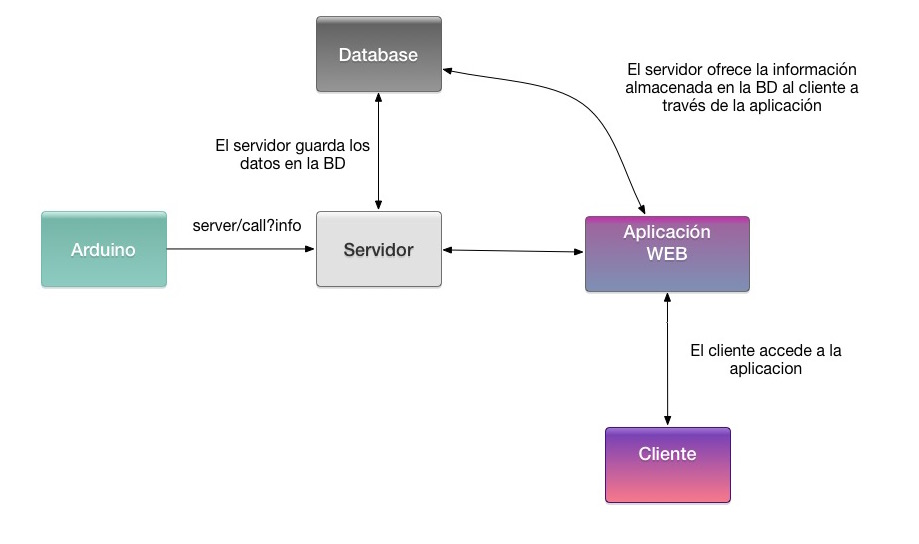
\includegraphics[width=0.9\linewidth]{figuras/montage1}
	\caption{Diagrama de montaje del proyecto en que función realizan las diferentes partes, desde el modulo hasta la información que podrá visualizar el cliente}
	\label{fig:imgnome}
\end{figure}



\section{Material}

Para este proyecto se ha utilizado el siguiente material:

Arduino Due: Es la Controladora que se encarga de recibir la información y procesarla para enviarla al servidor.

Ethernet Shield:

Modulo GPS NEO6mv2:

Sensores:

Cableado:

Servidor:




